% !TEX root = paper.tex
\iflong
\else
\vspace{-2mm}
\fi
\iflong
\else
\begin{figure}[hpt!]
\centering

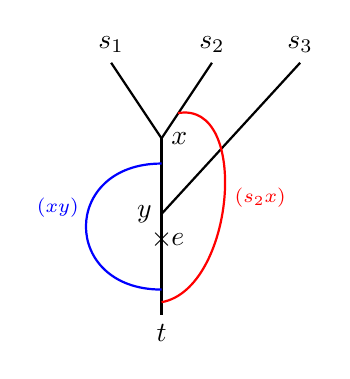
\begin{tikzpicture}[scale=1.6]
\begin{scope}
\coordinate (s2) at (0.4,2);
\coordinate (s1) at (-0.4,2);
\coordinate (s3) at (1.1,2);
\coordinate (x) at (0,1.4);
\coordinate (y) at (0,0.8);
\coordinate (t) at (0,0);
\coordinate (ts) at (0.15,0.4);
\coordinate (b1) at (0,.2);


\coordinate (a1) at (0,1.2);
\coordinate (a2) at (0.13,1.6);
\coordinate (v) at (0,.6);

\coordinate (c) at (-0.7,0.66);
\coordinate (b2) at (0,0.1);

\draw[thick](s1)--(x);
\draw[thick](s3)--(y);
\draw[thick](s2)--(x);
\draw[thick](x)--(t);
\node[above] at (s2){$s_2$};
\node[above] at (s1){$s_1$};
\node[above] at (s3){$s_3$};
\node[below] at (t){$t$};


\node[left] at (y){$y$};
\node[right] at (x){$x$};


\draw[blue,thick] (a1) to[out=180,in=180,distance=.8cm]
node[pos=0.4,left]
{\scriptsize  $\TON(xy)$}  (b1);



\draw[red,thick] (a2) to[out=10,in=10]
node[pos=0.5,right]
{\scriptsize  $\TON(s_2x)$}  (b2);

\node at (v){$\times$};
\node[right] at (v){$e$};

\end{scope}

\end{tikzpicture}
\caption{The shortest path from $s_2$ to $t$ avoiding $e$ can be $\TON(xy)$ or $\TON(s_2x)$.}
\label{fig:heavylight}

\end{figure}

\fi
\section{Building the Data Structure}
\iflong
\else
\vspace{-4mm}
\fi
\label{sec:data}

Let us first recognize a potential problem in using $\TON(\cdot)$.
%Consider a segment $xy$. We know that $\TON(xy)$ is a replacement path from $x$ to $t$ avoiding $yt_x$. We store only one path from $\TON$ for the segment $xy$   as
%we don't have enough space to store all the paths. However, this strategy leads to the following
%problem.
Let $s_1t$ and $s_2t$ path  meet at vertex $x$ (See Figure \ref{fig:heavylight}).
Another path $s_3t$
 meets $s_2t$ path at $y$ where $y$ is closer to $t$.
$\TON(s_2x)$ is the shortest path from $s_1$ to $t$ avoiding $e$ and $\TON(xy)$ is the shortest path from
$x$ to $t$ avoiding $e \in yt $. This immediately leads to the following problem. Assume that
the query is $\textsc{Q}(s_2,t,e)$ and the preferred path avoiding $e$ is in $\TON$.
Then there are two  candidate paths that avoid
$e$: one that goes from $s_2$ to the intersection vertex $x$ and then take
path  $\TON(xy)$ and the other $\TON(s_2x)$.
Thus, we need to check these two paths and return the minimum of the two. One can
make a bigger example in which there are $\sigma$ segments between $s_2$ and $t$
and thus we have to check $O(\sigma)$ path before we can answer the query. The problem appears
because we don't know from which segment the shortest path avoiding $e$ started its detour.
If this information is not there, then it seems that we have to look at all the segments between
$s_2$ ans $t$.
\iflong
\begin{figure}[hpt!]
\centering

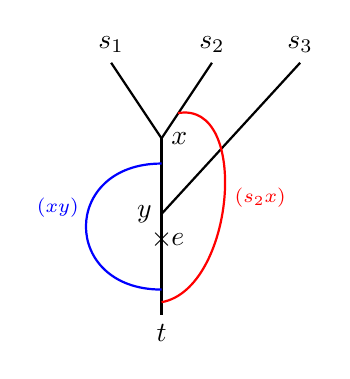
\begin{tikzpicture}[scale=1.6]
\begin{scope}
\coordinate (s2) at (0.4,2);
\coordinate (s1) at (-0.4,2);
\coordinate (s3) at (1.1,2);
\coordinate (x) at (0,1.4);
\coordinate (y) at (0,0.8);
\coordinate (t) at (0,0);
\coordinate (ts) at (0.15,0.4);
\coordinate (b1) at (0,.2);


\coordinate (a1) at (0,1.2);
\coordinate (a2) at (0.13,1.6);
\coordinate (v) at (0,.6);

\coordinate (c) at (-0.7,0.66);
\coordinate (b2) at (0,0.1);

\draw[thick](s1)--(x);
\draw[thick](s3)--(y);
\draw[thick](s2)--(x);
\draw[thick](x)--(t);
\node[above] at (s2){$s_2$};
\node[above] at (s1){$s_1$};
\node[above] at (s3){$s_3$};
\node[below] at (t){$t$};


\node[left] at (y){$y$};
\node[right] at (x){$x$};


\draw[blue,thick] (a1) to[out=180,in=180,distance=.8cm]
node[pos=0.4,left]
{\scriptsize  $\TON(xy)$}  (b1);



\draw[red,thick] (a2) to[out=10,in=10]
node[pos=0.5,right]
{\scriptsize  $\TON(s_2x)$}  (b2);

\node at (v){$\times$};
\node[right] at (v){$e$};

\end{scope}

\end{tikzpicture}
\caption{The shortest path from $s_2$ to $t$ avoiding $e$ can be $\TON(xy)$ or $\TON(s_2x)$.}
\label{fig:heavylight}

\end{figure}

\fi
To end this dilemma, we use heavy light decomposition of \SBFS($t$) \cite{SleatorT83}.
For any segment $xy \in$ \SBFS($t$) (by our convention $y$ is closer to $t$), $x$ is a {\em heavy}
child of $y$ if the number of nodes in the subtree under $x$ is $\ge$ 1/2(number of
nodes in the subtree under $y$) else it is called a {\em light child} (or light {\em segment} in our case).
%$x$ is also called the {\em heavy child} of $y$.
It follows
that each intersection vertex has exactly one heavy child and
each vertex is adjacent to atmost two heavy edges. A {\em heavy chain} is a concatenation of
heavy edges. A {\em heavy subpath} is a subpath of a heavy chain.
The following lemma notes a well known property of heavy-light decomposition.

\begin{lemma}
\label{lem:decomposition}
The path from a source $s$ to $t$ in \SBFS($t$) can be decomposed into $O(\log n)$ heavy subpaths
and light segments .
\end{lemma}

Given any source $s \in S$, by Lemma \ref{lem:decomposition},
the path from $t$ to $s$
may contain many heavy subpaths.
Let $C(pq)$ be a heavy
chain that starts at $p$
and ends at $q$ (where $q$ is closer to $t$ than $p$). A $ts$ path may follow
a heavy chain $C(pq)$ but may exit
this chain from a vertex midway, say at $r$. Let $(C(pq), r)$
be a tuple associated with $s$
such that the shortest path from $t$ to $s$ enters this
heavy chain via $q$ and
leaves this chain at $r$. We keep a list $\HE(s,t)$
which contains
all the tuples $(C(pq), r)$ sorted according to
the distance of heavy chain
from $t$ (that is distance $qt$). By Lemma \ref{lem:decomposition},
the size
of $\HE(s,t) = O(\log n)$. Similarly, we have one more
list to store the light segments.
$\LI(s,t)$ contains all the light segments on the $st$ path
again ordered according to their
distance from $t$ in \SBFS($t$). Again by Lemma  \ref{lem:decomposition},
the size
of $\LI(s,t) = O(\log n)$. Note that the size of these additional
two data-structures
is $\sum_{s \in S} O(\log n) = \tilde O(\sigma) = \tilde O(\sqrt{n\sigma})$.


Our main problem was that we have to find the minimum $\TON(\cdot)$ of $O(\sigma)$ segments if 
there is a path of length $\sigma$ between $s$ and $t$. The trick we use here is that
finding minimum on any heavy subpath takes $\tilde O(1)$ time. Since
there are $O(\log n)$ heavy subpaths, the total time taken to find the minimum
on heavy subpaths in $\tilde O(1)$. Also, since the number of light segments is also $O(\log n)$
finding the minimum among these also takes $\tilde O(1)$ time.

We now describe our intuition in detail.  Let $xy$ be a segment in a heavy chain
$C(pq)$. We want to represent $\TON(xy)$ in a
balanced binary search tree $\BST(C)$. To this end, we will add a node with
the tuple $(x.depth,| px \conc \TON(xy) |, |px|)$  in $\BST(C)$.
The first element in this tuple is the depth of $x$
in $\BFS(t)$ --  it also acts as the key in this binary search tree. The second element
is the path $ \TON(xy)$  concatenated with $px$. This concatenation is done so that all  paths
in $\BST(C)$ start from $p$ and comparing two paths in $\BST(C)$ is
possible. The third element will be used to get the path length $\TON(xy)$ (by subtracting it from
the second element) when
need arises. Now we can augment
this tree so that the following range minimum query can be answered in $\tilde O(1)$ time:
$\RMQ(C(pq),[a,b])$ : Find minimum of $\{|px \conc \TON(xy)|\ |\ xy \ \text{is a segment in heavy chain $C(pq)$ and }\ x.depth \ge a.depth \ \text{and}\  x.depth \le b.depth \}$.
The size of $\cup_{C \in \HE(s,t)}\BST(C)$ is $O(\sigma) = O(\sqrt{n\sigma})$ as there are
at most $O(\sigma)$ segments in \SBFS($t$).
\iflong
\begin{algorithm}
\SetKwRepeat{Do}{do}{while}%
  \caption{Finding the shortest replacement path  (in $\TON$) from $s$ to $t$ avoiding $e(u,v)$ }
  \label{fig:findR1R2}
Let $x$ be  the first intersection point on $us$ path\;
$min \leftarrow \infty$ \;

\Do{$x$ is not equal to $s$ }
{
    \If{ $x$ lies in a heavy chain}
    {
        Using $\HE(s,t)$, find $(C(pq),r)$, that is $r$ is the vertex from which $us$
        path leaves the chain $C$\;
        $min\leftarrow \min\{ min, \RMQ(C, [x,r]) - |pr| + |sr| \}$\;
        $x \leftarrow r$\;
    }
    \ElseIf{$x$ is an endpoint of a light segment}
    {
        Let $x'x$ be the  light segment ending at $x$ in \SBFS($t$) \tcp*{Can be found out via $\LI(s,t)$ in $\tilde O(1)$ time.}

        $min \leftarrow \min\{ min, |\TON(x'x)| + |sx'| \}$\;
        $x \leftarrow x'$\;
    }
}
\end{algorithm}
\fi


Given any edge $e(u,v)$ on $st$ path, we can now find the shortest path in $\TON$ from
$s$ to $t$ avoiding $e$
\iflong
(see Algorithm \ref{fig:findR1R2}).
\else
(Please refer to Algorithm \iflong\ref{fig:findR1R2}\else 1\fi~ in the full version of the paper).
\fi We first find the first intersection vertex on the
$us$ path from $u$. Let this vertex be $x$. We will see that finding
$x$ is also not a trivial problem --  we will say more about this problem later.
Now, we will go over all  possible replacement paths from $u$ to $s$.
Thus, we  search if there exists any heavy chain in
$\HE(s,t)$ that contains $x$. To this end, we first check if $x$ lies in some light segment (this can be checked in $\tilde O(1)$ time). If not, then $x$ lies in some heavy chain. We now search each heavy chain in $\HE(s,t)$ to find a node $x'$ with the smallest depth such that  $x'.depth > x.depth$.
Let this node be $x'$. Thus we have found the segment $x'x$ where $x$ is closer to $t$
than $x'$.
%where $x.depth$ is the depth of $v$ in $\BFS(t)$.
We can easily calculate $x.depth$ as
$|st| - |sx|$ or $B_0(s,t) - B_0(s,x)$. Since there are $\tilde O(1)$ heavy
chain in $\HE(s,t)$, the time taken to find if $x'x$ exists in some heavy chain is $\tilde O(1)$.
%Similarly, the reader can infer that the time taken to %find the light segment
%in which $x$ is an endpoint is $\tilde O(1)$.
%Once we have found such a
%heavy path or light segment, then we check if the replacement %lies on it.

Assume that we found out that
$x'x \in C(pq)$,  and $ts$ path leaves the chain $C$ at $r$, then we want to
find the shortest replacement path from $r$ to $t$ avoiding $e$. This can be found out via the range minimum query $\RMQ(C(p,q),[x,r])$.
However, note that each replacement path in $C$ starts from $p$. So, we need to
remove $|pr|$ from the replacement path length returned by $\RMQ$ query.
The length $pr$ can be found out in the node $r \in \BST(C)$. Finally, we add $|sr|$ to get the path from $s$ to $t$.

Similarly, we can process a light segment in $O(1)$ time (please refer to Algorithm \iflong\ref{fig:findR1R2}\else
1 in the full version\fi~).
Thus, the time taken by  Algorithm  \iflong\ref{fig:findR1R2}\else
1\fi~ is
$\tilde O(1)$ as the while loop runs at most $O(\log n)$ times  and each step in
the while loop runs in $\tilde O(1)$ time.



%The above algorithm moves from vertex $u$ to $s$, that is $us$ path.
%If it encounters a light edge $vv'$ in this path then it, then we check if the
%$st$ path whose detour starts on $vv'$ is the minimum, that is path $sv' \conc \TON(v')$.
%Else, if we encounter a heavy chain, then we

\begin{comment}
We are now ready to describe our data-structure to process queries. We first need
to check the vertex to be avoided is an intersection point in \SBFS$(t)$. To this end,
we check if the vertex exists in $\BST_1(t)$. If yes, then we return the length of the
preferred path associated with the vertex. The size of
$\BST_1(t)$ is $O(\sigma) = O(\sqrt{n \sigma})$ as there are $O(\sigma)$ intersection
point in \SBFS$(t)$.


Let $xy$ be a segment in \SBFS$(t)$.  We will associate two data structures with
$x$, (1) $D_0(x,t)$ contains   the preferred replacement path from $x$ to $t$
such that its detour starts in segment $xy$, but the avoided vertex lies in $yt$,
that is, that path in $\TON$ (2) $\BST_2(x,t)$ contains all the  preferred path
from $x$ to $t$ such that their detour start in segment $xy$ and the avoided
vertex also lies in $xy$, that is, paths in $\TTW$. As in the single source case,
we first show that each path in $\BST_2(x,t)$ avoid a contiguous subpath of $xy$.

By Corollary \ref{cor:arrange}, we can arrange paths in $\BST_2(x,t)$ in decreasing order of their length. By
Lemma \ref{lem:avoids}, for any two path $P,P' \in \BST_2(x,t)$, if $|P| > |P'|$, then $\DET(P')$
starts below the vertex avoided by $P$. This lemma implies
that $\DET(P')$ starts below all the vertices avoided by
$P$. Thus $P$ avoids some contiguous path in $xy$ path.
We can $\BST_2(x,t)$ as a balanced binary search tree. For each subpath $zz'$ of $xy$,
we store the length of the replacement path from $x$ whose detour starts before $z$ and it
meets $xt$ path again in $t_xt$.  Additionally, we also store the distance of $z$ and $z'$
from $x$. These distances will act as the key of a node in $\BST_2(x,t)$.
\end{comment}
\iflong
\else
\vspace{-2mm}
\fi
\subsection{Answering queries in $\tilde O(1)$ time}
\iflong
\else
\vspace{-2mm}
\fi
Given a query ${\sc Q}(s,t,e(u,v))$, we process it as follows
(assuming that $e$ lies on $st_s$ path (that is the {\em far case)} and $v$ is closer to $t$ than $u$)\iflong\\\else\vspace{1mm}\fi


\begin{comment}
{\em (1) Check if $e$ lies on $st_s$ path.}

  Since all the shortest path have unique length, we find if $|su|_{p} + |ut_s| _{p}+ |t_st|_{p} = |st|_p$. To this end, we use the data structure already defined in Section \ref{}. We first find $t_s \leftarrow
  B_2(s,t)$.
  Then we check if $B_0^{p}(s,u) +\ B_0^{p}(u,t_s) +\ B_0^{p}(t_s,t)
  = B_0^{p}(s,t)$.

  \item Check if $u$ is an intersection vertex in \SBFS$(t)$.

  For each $t$ we build a balanced binary search tree that stores all the intersection vertex in $\BFS(t)$. Since the number of intersection vertex in $\BFS(t)$ is $O(\sigma)$, the size of this binary search tree is $O(\sigma) = O(\sqrt{n \sigma})$. We then check now check  $u$ is an intersection vertex in  $\tilde O(1)$ time.

\end{comment}

\begin{enumerate}[leftmargin=*,noitemsep,nolistsep]
\item Find the first intersection vertex  on $us$ path.

\iflong
  \noindent As we have mentioned before, this is not a trivial problem.
  Let the first intersection vertex from $u$ to $s$ in $\BST(t)$ be
  denoted by  $\INT_{s}(u,t)$.   We will first show that $\INT_{s}(u,t)$ is independent of $s$.
  \begin{lemma}
  \label{lem:intlemma}
  $\INT_s(u,t) = \INT_{s'}(u,t)$ for $s,s' \in S$ for all $u \in \BFS(t)$.
  \end{lemma}

  \iflong
  \begin{proof}
    We will prove this by induction on the nodes of $\BFS(t)$ from leaf to root $t$.
    The base case is a leaf in $\BFS(t)$, that is a source vertex, which by definition,
    itself is an intersection vertex. For any node $u$, if $u$ is an intersection vertex,
    $\INT_s(u,t) = \INT_{s'}(u,t) = u$. Else, $u$ is a node of degree 2 in $\BFS(t)$.
    Assume that $u'$ is the child of $u$ in $\BFS(t)$. So, $\INT_s(u,t) = \INT_s(u',t)$ and $\INT_{s'}(u,t) = \INT_{s'}(u',t)$. But by induction hypothesis,  $\INT_s(u',t)=\INT_{s'}(u',t)$.

    \end{proof}
  \fi

  \noindent We will drop the subscript $s$ from the definition of $\INT(\cdot,\cdot)$ as we now know that it is independent of $s$. We use the
  above lemma to construct  two data structures that will help us in finding $\INT(u,t)$.

  \begin{itemize}
  \item $I_1(t)$: For any $u \in V$, if $\INT(u,t)$ is within a distance of $c\sqrt{n/\sigma} \log n$
  (for some constant $c$) from $u$, then we store the tuple
  $(u,\INT(u,t)$) in the balanced binary search tree $I_1(t)$. For any  intersection
  vertex $x \in $ \SBFS$(t)$, we  store at most $\tilde O(\sqrt{n/\sigma})$ tuples in $I_1(t)$.
  For a fixed $t$, the total
  space taken by $I_1(t)$ is $\tilde O(\sigma .\sqrt{(n/\sigma)}
  )= \tilde O(\sqrt{n \sigma})$ (as there are $O(\sigma)$ intersection vertices in \SBFS($t)$.
  %Given a vertex $u$, we then try to find if $u$
  %exists in this data-structure. This takes $\tilde O(1)$
  %time.

  \item $I_2(t)$: If $u$ is not present in $I_1(t)$, then $\INT(u,t)$ is at a distance
  $\ge c\sqrt{n /\sigma}\log n$ from $u$. We now
  use a different strategy to find $\INT(u,t)$. We first find $u_s \leftarrow B_1(s,u)$,
  that is the vertex in $\TT$
  closest to  $u$ in $su$ path. With a
high probability,
$u_s$ is closer to $u$ than $\INT(u,t)$ and all the vertices from $u$ to $u_s$ have degree  exactly 2 in $\BFS(t)$.
  Thus, $\INT(u_s,t) = \INT(u,t)$ -- we will now use this property (a similar property was also used in the proof of Lemma \ref{lem:intlemma}).

  \begin{comment}
        \begin{figure}[hpt!]
        \begin{algorithm}[H]
        \If{$u \in I_1(t)$}
        {
            return $I_1(u,t)$;
        }
        \Else
        {
            $u_s \leftarrow B_1(s,u)$\;
            return $I_2(u_s,t)$;
        }
        \end{algorithm}
        \caption{\textsc{Find-Int}$(s,u,t)$: An algorithm to find $\INT_s(u,t)$}
        \end{figure}
  \end{comment}
  \noindent
  For each $x \in \TT$
  such that $x$ is not an intersection vertex in $\BFS(t)$, we store the tuple
  $(x,\INT(x,t))$ in another balanced binary search tree $I_2(t)$. For a fixed vertex $t$, the
  size of this data-structure is $\tilde O(\sqrt{n\sigma})$ space
  as there is only one intersection vertex for each vertex
  in $\TT$ and $|\TT| = \tilde O(\sqrt{n \sigma})$

\end{itemize}
  \noindent If $\INT(u,t)$ is indeed at a distance $\le
c \sqrt{n / \sigma} \log n$,
  then we can use $I_1(t)$  to find it in $\tilde O(1)$
time, else we use $I_2(t)$ to find
  $\INT(u_s,t)$ in $\tilde O(1)$ time.\\

  \begin{comment}
  \noindent {\em Assuming $x = \INT_s(u,t)$,  find $\INT_s(x,t)$}

  Our aim is to find the segment which ends at $x$ in \SBFS($t)$. To this end,
  we find $\INT(x,t)$. To this end, we use another balanced binary search tree.
  For each intersection vertex $v \in $ \SBFS($t$), we store the tuple
  $(s,\INT_s(v,t))$ in $I_3(v,t)$. Unlike non intersection vertex, for an
  intersection vertex $v$, $\INT_s(v,t)$ may be dependent on $s$.

  \end{comment}
\else
\noindent In the full version of the paper, we show that we can find the first intersection vertex  on $us$ path
in $\tilde O(1)$ time using $O(\sqrt{n\sigma} )$ space.
\fi
\item Find  the replacement path avoiding $u$  if it lies in $\TON$.
\label{fcase1}

\noindent To this end, we use our Algorithm \iflong\ref{fig:findR1R2}\else
1\fi.
The first non-trivial part of this algorithm, that is, finding the first
intersection vertex on the $us$ path has already been tackled in the point above.
So we can find such a replacement path (if it exists) in
$\tilde O(1)$ time  and $\tilde O(\sqrt{n \sigma})$ space.\iflong\\\else\vspace{1mm}\fi


\item Find the replacement path avoiding $e(u,v)$ if it lies in $\TTW$.
\label{fcase2}

\noindent  This part is similar to our data-structure in single source case.
Let $x \leftarrow \INT(u,t)$.  Using $\HE(s,t)$ and $\LI(s,t)$, in $\tilde O(1)$ time,
we can find the segment $xy \in $ \SBFS($t$) such that $y$ is closer to $t$ than $x$.
In this case, we want to check if there exists any
replacement path that starts in  the  same segment in which
$e$ resides. This  replacement path first takes $sx$ path and then takes
 the  detour strictly inside  the  segment $xy$. All such paths are stored in $\TTW(xy)$
with the contiguous range of edges that they avoid on $xy$.
We now just need to check if $u$ and $v$ lie in the range of some replacement path.
To this end, we find $u.depth \leftarrow |st| -|su| = B_0(s,t) - B_0(s,u)$
and $v.depth \leftarrow |st| -|sv| = B_0(s,t) - B_0(s,v)$.
Now we check if $u.depth$ and $v.depth$ lie in contiguous range of
some replacement path  in $\TTW(xy)$. If yes, then we return the length of that
path concatenated with $sx$.  Note that we have already stored $|sx|$ in $B_0(s,x)$.
The time taken in this case is dominated by searching $u$ and $v$ in $\TTW(xy)$,
that is $\tilde O(1)$.\iflong\\\else\vspace{1mm}\fi
\end{enumerate}

\noindent Thus, the total query time of our algorithm is $\tilde O(1)$, and we can return the
minimum of replacement paths found in Step \ref{fcase1} and \ref{fcase2} as our final answer.
The reader can check that the space taken by our algorithm for a
vertex $t$ is $\tilde O(\sqrt{n\sigma})$. Thus the total space taken by our algorithm is
$\tilde O( \sigma^{1/2} n^{3/2}) $. Thus we have proved the main result, that is Theorem \ref{thm:maintheorem} of our paper.

%\begin{theorem}
%There exists a data-structure of size $\tilde O(\sigma^{1/2}n^{3/2})$
%for multiple source single fault tolerant exact distance oracle
%that can answer each query in $\tilde O(1)$ time.
%\end{theorem}
